\section*{}

\begin{minipage}[t]{.48\textwidth}
  \vspace{0pt}

\end{minipage}
\hfill
\begin{minipage}[t]{.48\textwidth}
  \begin{flushright}
    ``\emph{Du siehst, mein Sohn,\\
      zum Raum wird hier Zeit.}''\\
    \vspace{0.5cm}
    ``\emph{You see, my son,\\
      time here becomes space}''
  \end{flushright}
  \flushright{\small{Richard Wagner, \emph{Parsifal}, act I}}
\end{minipage}
\vspace{1cm}


\section{Introduction}
\label{sec:introduction}

\noindent
This chapter discusses the challenges related to arts-based research in and through time-based artistic expressions. Even though the focus is on musical practice, specifically interactive music, it is fair to assume that some of these challenges discussed are common to several other real-time scenic and performing art forms. A point of departure is that the needs put forward by these fields of artistic practice are not necessarily synchronous to those deployed by the non-real time arts.\footnote{It should however be noted that few art forms are unanimously non-real time or real-time. As far as time is concerned, music genres such as electro acoustic tape music---music produced electronically, recorded unto tape or disc and played back from the same---is conceptually close to non-real time art forms. Furthermore, the visual arts encompasses activities that that are highly dynamic and depend on real-time in ways similar to the ways music does traditionally.} Furthermore it is suggested that there is a difference between a reflection upon the research object as a whole and a reflection of the research object as it unfolds in time. Therefore, it is argued, the researcher engaged in arts-based research in the real-time arts should embrace and investigate the in-time properties of the research object. Finally a point is made that, due to the complex nature of in-time processes, the outcome of an arts-based research that investigates the temporal flow of the object in time may be of interest also outside the art world. 

The fact that in music \emph{action} takes place \emph{in} and \emph{through} real time rather than primarily \emph{over} time makes it an interesting, and equally difficult, candidate for artistic research. To gain access to whatever information may be hidden in its in-time properties the researcher need to resist the temptation of falling back on the investigation of the over-time and out-of-time representations of (only) the art work, such as musical scores, manuscripts, transcriptions, etc. Although most musical expressions offer the same temporal complexity, in the practice of Interactive Music, which is briefly discussed in Section \ref{sec:why-interaction}, the man-machine interactions surfaces the in-time aspects of music in a particularly useful way. As an hint at the compound nature of time, in Section \ref{sec:performing-time} a brief overview of temporal multiplicities is given.
% as well as an example of an outside of time, in-memory representation of events unfolding in time. 
In Section \ref{sec:performing-practice} the artistic practice of the author is used to exemplify the research process from within the musical flow and the feedback between the different aspects of the practice. By turning to Bergson's important writing on memory, in Section \ref{sec:inter-with-virt} it is suggested that even the in-memory (virtual) representation of in-time processes contain and depend on time.

\section{Music and interaction}
\label{sec:why-interaction}

My primary interest, here and in general, is that which is commonly referred to as \emph{Interactive   music}; music where musicians interact with computers and other kinds of machines in real-time. The intricacy of the dynamics in the relationship between the man and the machine is of particular interest while working in the field of Interactive Music, and it is a practice that has a much wider scope considering the great challenges computer interface designers are facing and will face in the future as computers pave their way into new objects. The dissimilarity in the way in which man and machine deal with time and memory in, may be understood from the point of view of an \emph{in-time} versus \emph{over-time} continuum. The distinction between activities that take place \emph{in} time and those that takes place \emph{over} time is brought forward in a short report by cognitive scientist Tim \citeauthor{smithers96}.\footnote{I am indebted this reference to Vijay Iyer who is referring to it in a discussion on embodiment in improvisation. See \cite{iyer08} For the original source along with a few additional on the topic of robotics and cognitive science, see \cite[See][]{smithers96,vangelder98,smithers:98}} Actions that take place in time are actions where the time taken matters, where time is a factor whose value is decisive. For example, when I walk it is not just that my leg is moving that matters but also the time it takes to move it. As for actions that occur over time, the time consumed by the action is of little significance for the result. Computation is a typical example of an over-time operation: The primary interest is the result itself, and as such it will not be affected by the amount of time it takes to arrive at it. Much (but not all) of art production, at least in its early stages, are over-time activities as well as most other abstract operations. Painting a picture, conceptualizing an art installation or writing a musical score are over-time operations even if the result, or the instantiation of these art works are in-time operations. Musical performance and improvisation are typical in-time operations: They are \emph{embedded in time} (to use \citeauthor{smithers96} expression) whereas over-time operations may be said to be \emph{contained in time}. Along with advances in computer science and robotics, real time computation has altered the picture somewhat, but the difference between an over-time operation being so fast that time goes unnoticed is very different from the way the mind ``exploits both the constraints and allowances of the natural timescales of the body and the brain as a total physical system.''\footcite[276]{iyer08} The in-time versus over-time distinction is interesting with regard to the topic of time and temporality, but it is also of interest to the specific topic of Interactive music. As a genre, Interactive music descend from Computer Music, also called Electro-acoustic music, and has strong interdisciplinary connections with subject areas such as Artificial Intelligence, Cognitive Science and Computer Science.\footcite[24]{moore90} These disciplines are concerned with trying to understand human behavior and, to some extent, attempt to mimic that behavior in machines. In the context of arts-based research it is important to draw upon knowledge that emanates from related fields of inquiry but it is equally important to re-evaluate those same sources. Historically there may have been a tendency for Computer music to lean against the natural sciences that, in fact, may also have much to gain from learning from the artistic practice of Computer music. The concept of time in general and the in-time aspect of music in particular.

When the technology became usable in the early 90's, Virtual Reality was seen as a great potential for art production.\footcite[See for example]{moser96,wood98,dixon07} The virtual reality is a game of deception where there is no extension in space (although there appears to be one) and where existence depends entirely on the interactions of the subject with the virtual reality technology. The virtual is disembodied and it is furthermore truly non-ocular in its complete absence of a consented visual component. After all, that is one of its great qualities; the users are able to mold their own (virtual) visuality.\footcite[Compare to William Gibson's definition of Cyberspace as a ``consensual hallucination''][51]{gibson84} This visuality may be different each time. Or, it may be identical to any other visuality, since making duplicates is no problem in the digital realm of the virtual. As technolgy has advanced its positions in Western culture, the virtual is nearly ubiquitous. To define a virtual reality that is distinct from reality is almost not possible. There is a virtual aspect to almost all activities in the occidental World.\footnote{\cite[See][]{baudrillard02:screened}. I also write about the topic of the real versus the virtual in interactive music in \cite[ch. 4]{frisk08}}

The virtual world offered to us by modern technology is interesting from the point of view of Arts Based Research, both in the ways that it deviates from the real world, but also in the ways that it connects Art and art practice to aberrant practices such as Computer Science and Artificial Intelligence. Thanks to their ignorance of conventions and lack of long term memory and historical insights, machines are phenomenal individual forgetting devices.\footcite[See][]{miller04} The absence of an embodied relation between the machine and its operator is further consolidating the breach between human cultural heritage and the agnostic nature of the machine. In the virtual world nothing is hard wired, hence, muscular memory is useless: Any one physical movement can have a different meaning each time.\footnote{The synthesizer is the perfect example here: Though it looks like a piano keyboard, any key can produce any imaginable (machine) sound, and a different one each time, all depending on how the synthesizer engine is programmed. Hence, any physical, embodied knowledge a trained pianist has with regard to sound production is virtually useless while playing a synthesizer or a keyboard attached to a computer instrument.} Envision the four members of Kraftwerk,\footnote{See \url{http://kraftwerk.technopop.com.br/pictures\_80years.php} for some pictures from live concerts, in particular the image from the TV show `Na Sowas' from 1982 is significant.} standing still and expressionless in front of their keyboards (obviously exploiting this dissociate aspect of their relation to the machine-instrument). Compare this vision to the physicality of almost any acoustic instrument performer playing live in front of an audience. The lack of context particular to the virtuality of electronic music---an electronic instrument may be updated and revised after which integral aspects of it has been altered---is an asset, but it is also a great frustration to some.\footcite[E.g.][]{ostertag02} At best it enables novel approaches to artistic problems or issues and at worst it creates expressions void of inter-musical (or inter-artistic) references. Approaching this field as a researching musician is a difficult task and the scientific as well as the social and cultural aspects of the virtual should be taken into consideration. How can the (non-)spaces of the virtual be truthfully represented outside its own domain? How may it be documented and communicated in the context of arts-based research?

When dealing with real-time technologies in music these questions are again brought to the fore. The real-time `object', the music that is a result of real-time processes such as improvisation, live coding, interpretation, etc., is made up of a volatile substance that is not easily transformed to a researchable `object'. While investigating how the virtual sound worlds of computer instruments, created and edited in real-time, may interact with (or fail at interacting with) the real world, the questions pertaining to access and documentation will become important. 
Although the Western tradition has developed powerful musicological methods to represent and document music visually,\footcite[See]{bregman94} independent of time, are there methods that retain the temporal identity of the object rather than do away with it? Such methods should also include questions rarely explored in arts-based research, such as the impact of contextuality and listener reception in musical and scenic performances. Also more multi disciplinary research projects will be of great interest here, in particular those that actively deal with visuality in different forms such as computer games and film. 

The aspect of interaction in the field of interactive art and media is problematic as the term \emph{interactive} to some extent has been hijacked by computer interface designers.\footnote{Susan Kozel similarly comments how the meaning of the word `virtual' is to be found when its ``overly reductive association with immersive technologies and that now anachronistic term cyberspace'' is removed.} Though one of its lexicographic meanings is ``Reciprocally active'',\footnote{``interactive, \textit{a}.'' The Oxford English Dictionary. 2nd ed. 1989. OED Online. Oxford University Press. 1 Nov. 2007. \url{http://dictionary.oed.com/cgi/entry/50118746}} its meaning in the context of computer interface design is more geared towards a methodology of control, than sharing, or mutual exchange. In the reduced meaning of computer interaction the actions of one part, `the user', is used to control the \emph{re}actions of the other, `the machine', often in a one-to-one relation: one action, one re-action. In this kind of interaction, a reaction to any given action is ignorant to any prior actions or reactions. A mouse click on a given icon on a computer desktop typically results in the same machine response, regardless of the user's preceding activities.

Musical interaction on the other hand is all about reciprocity, particularly in improvised music.\footcite[See for example][]{monson96} A successful interplay between musicians involved in an improvisation rests on a mutual sensitivity for taking, and responding to, musical initiatives. Musicians induce differences rather than alter states; they induce differences that ``\emph{make a difference}''.\footcite[And, according to Gregory Bateson, a difference that makes a difference is the definition of \emph{Information}][92]{Bateson} Even for an orchestra conductor---who is commonly seen as the \emph{director} of the music, commanding its flow---the agency of control is limited to what can be achieved through interaction with the musicians in the orchestra. Interaction-as-control and interaction-as-difference are not clear cut definitions in binary opposition. Again we are dealing with a continuum; a continuum of interactive potential ranging from the most reduced form of interaction-as-control (click and response) to the infinitely complex interaction-as-difference (e.g. musical interaction). 
The activity of playing back a CD-recording of a symphony on a sound system is an example of the former while conducting a symphony orchestra playing the same symphony is an (extreme) example of latter. What one may gain in control with the CD player, the recording and the sound system---a CD can be paused, repeated, removed, etc.---we loose in influence over content. 
As conductors we may alter the music in ways that we see fit, limited merely by cultural and social practices. But what we gain in influence in this context we loose in control: We can not as easily pause a live performance, considerable financial resources needs to be deployed in order to gather all the musicians needed, the training needed to be able to conduct a symphony orchestra is counted in years whereas the training needed to play back a CD is counted in seconds, etc.


\section{Time and multi temporality}
\label{sec:performing-time}

Performing music takes place \emph{in} time and I believe it is fair to assume that there is a difference between investigating `the object'\footnote{Let the object, for the moment, encompass all and any aspects of the artistic practice.} in-time, while it is unfolding, as opposed to doing it over-time. A researching musician needs to be able to explore the object in a multifaceted way, as a stratum of analytical modes in simultaneous operation. The question of time is significant as many of the different processes involved simultaneously take place in  different time scales or temporal modes. While performing the musician measures the perceived sound against an inner vision of what was intended, and against prior performances, and this evaluation is constantly performed at different temporal resolutions. Orchestra conductors are making judgments on the music in the present based on their knowledge and expectation of what will happen in the future of the music: in next bar, the next section, the next movement, the end of the concert, the next concert, etc. They are able to constantly keep a fish eye view on the piece without loosing the details in the process. The conductor is accessing the object at different rates and at different temporal locations, or points in history (and in the future), all at the same time. 

A number of composers and theorists have stressed the multiplicity of temporal modes present in music and the American electronic music composers Curtis Roads makes the interesting remark that the discontinuities that appear in the boundaries between different time scales gives rise to perceptual differences in sonic events.\footcite[4]{roads}  A note terribly out of tune in one temporal order may have just the right intonation in another, and a beat out of sync in one time scale may swing in another.\footcite[For an example of the great variation in rhythmic timing among jazz musicians when observed at high temporal resolution, see][]{friberg02} 

To the Greek composer and architect Iannis Xenakis the discontinuity of time was of pivotal import. Not only the interruptions that occur when moving across the boundaries between different temporal scales, but also the separability of events occurring within the flux of one particular time scale. According to Xenakis, non-synchronicity and discontinuity of events in time is what makes the flux of time perceptible: Without it time would remain hidden, illegible and inapproachable. Painting a picture of chains of events that makes time come forward, Xenakis also argues that their representation in the brain---our memory of events in time---is a generalization and abstraction that exists outside of time: ``Memory is the spatial translation of temporal (causal) chains.''\footcite[263]{xenakis71} 
Contiguous events, separate in time, creates durations in the flux of time and marks out spatial distances in its memory representation: Time becomes space. Following this line of thought, music is an art form that, in most cases, participates in space as part of a temporal flux. It lays out events in the flow of time, a flow which in itself, in some cases, is controlled by these events. But, according to Xenakis, at the same time, the same music, also exist outside of time as a snapshot, as an abstract representation.
This representation, when encoded in our memories, or when described as a musical structure (e.g. a fugue), becomes accessible to us as a whole. A whole which we can navigate, jump back and forth in, and sustain at random access. The whole becomes, not a succession, but something non-temporal that ``can be viewed as one \emph{time spectrum} of a fundamental duration''.\footnote{\cite[73, my italics.]{roads} See also \cite{stockhausen57}}
That in-time processes such as music are transformed to images or gets spatialized in the human brain is a common thought, but the fact that Xenakis uses the idea of a time \emph{spectrum} is interesting. When the frequency spectrum of a sound is calculated using a Fourier Transform, increasing the resolution in frequency reduces the temporal resolution, and vice versa. It is not easily possible to simultaneously retain high frequency resolution \emph{and} high temporal resolution. In the time spectrum that Xenakis is talking about, a whole in which an entire compositional structure is encoded, there is a similar trade-off between temporal resolution and spectral resolution. Returning to his claim that memory is a spatial translation of contiguous events in time: Perhaps it is to be seen as a spatial spectrum of a fundamental duration, a way to look at the structure as a function of space rather than a function of time. The time spectrum---which should really be called a \emph{space} spectrum---transforms events in time to events in space, and the reverse transforms spatial properties in events to temporal properties. Thoughts like these may seem speculative; as abstract constructs induced on top of an artistic expression. But when, and if, they are the result of research performed from within the artistic practice, they may carry with them novel ideas, specifically about the concept of musical time, but also with regard to time and memory in general.

Perhaps Xenakis' idea of a musical memory as a spatial translation of the musical events contained in it should be traced to his background as an architect, and is influenced by his aptitude and sensibility for spatial rendering. If we limit ourselves to the realm of the time based arts, is it really possible that our in memory representation of something such as music, that exists and evolves in time, can be represented independent of time? And if it is, what is the coupling between time and space that makes the transformations from one to the other transparent; how is the space/time spectrum calculated? These are examples of questions that may be tackled from within an artistic practice in the context of arts-based research. Only from within the flow of time is it possible to fully grasp the time-space transformations and their significances, specifically as well as generally. Furthermore, the results of such an interrogation performed from within, are likely to be different from those obtained from the outside, and hence they have the potential to contribute new knowledge to several fields if inquiry.


% In music, many different time scales are active, influential and % operative simultaneously and it is possible, for the listener as well % as for the performer, to move between them. Although it is true that % this movement alters the listeners perceptions, the moving between % timescales and the coexistance of multiple timescales is also possible % without the discontinuity brought up by \citeauthor{roads} above. 

\section{Performing in practice}
\label{sec:performing-practice}

Something that is embedded in time will always be difficult---but not impossible--to conceive of as an object (though object is a misleading term here), independent of its temporal context. Despite Xenakis' argument to the contrary, as was discussed in the previous section, this `object' will not easily transform itself to a spatial representation along the lines of what was discussed above, because it is not just the order of events and the speed at which they are deployed that matters and that gives this object its character. The performer/researcher working in the field of arts-based research should resist the temptation of objectifying the in-time performance and instead embrace the possibilities and the great challenges that lies in investigating the in-the-moment, unfolding, real-time, processes of creative and interactive activities. These depend on properties that will not transform themselves to out-of-time representations without something substantial being lost. Their in-time aspects, such as their physicality, and intersubjectivity, are primarily accessible from the inside, from within the creative activity and they will risk at loosing their identity if resolved of their `in-timeness', if they are instead looked upon as over-time processes. Aiming at performing research in time is a difficult task but I will argue that for arts-based research in time based arts to be different from e.g. standard musicological research, it has to face these difficulties and attempt at accessing the object form the inside and research the in-time object as it is unfolding. The means to do it and the methods to use will inevitably have to differ from case to case and from discipline to discipline but investigating and acknowledging the difference between divergent temporal domains and temporalities is a prerequisite, regardless of the discipline. In other words, to engage in arts-based research, accessing the object of research as an in-time process constitutes an activity that may offer an interesting alternative to the otherwise dominating visual modes of research expressions. Discussing the practice of an improvising musician without resorting (solely) on transcriptions of the performances, or other abstract representations, is likely to render a result different from traditional musicological research, or arts-based research that primarily takes place outside the temporal flow of the object. To visualize a flow of time, i.e. to perform the kind of time spectrum transformation as was suggested by Xenakis above, is admittedly a powerful and pedagogical conjuration\footnote{A popular example is the famous scene in Hitchcock's 1959 movie \citetitle{hitchcock59}. Madeleine (played by Kim Novak), whose identity is overwhelmed by her great grand-mother, is standing in front of a cross section of an over 1000 years old Redwood tree. She places her finger towards the outer ring of the tree and marks out the point where she was born and the point where she died. The distance between the two points is short relative to the size of the tree, and, as she is moving her finger across the wood, she says ``It was only a moment to you''. \cite{hitchcock59} The cross section of the tree is used to spatialize a (short) life span, to transform a duration to a distance, to transform time to space. Another, similarly schizophrenic, example is the end of the first act of Richard Wagner's opera Parsifal (cited above) where there is a slightly more subtle and continuous transformation from time to space. Parsifal makes a remark that, despite his slow pace he already seem to have come far. The explanation offered to him is that ``time here becomes space''. \cite[See][act 1]{wagner82}} but it is equally deceptive: It is a transformation of an in-time process to an over-time process, and in the shift, temporal as well as other kinds of information is bound to get lost.


\begin{figure}[htb]
  \centering
  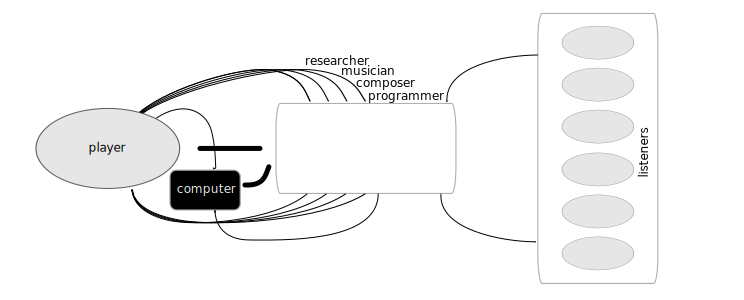
\includegraphics[width=\linewidth]{img/player-computer}
  \caption{\small{A simplified graphic representation of an instant of an improvised performance with an interactive computer. The performer is reflecting upon the output in several different modes of thinking (represented by the arrows leading from the performer to the sound). The feedback of the reflection and its influence on the object is represented by the arrows leading from the object back to the performer.}}
  \label{fig:player-comp}
\end{figure}

As a performer, engaged in an actual performance with an Interactive computer system, and simultaneously a researcher, I obviously combine several different roles and disseminating processes at once. As can be drawn from the graphic in Figure \ref{fig:player-comp} I at once access and evaluate the object in different modes of thinking relating to the different tasks I carry out, or have carried out in preparation for the performance (programmer, musician, composer, etc.). The object in this case is simplified to constitute the bare audible (poietic) trace left by what I and the computer produce together. Similar to how it was noted with regard to the conductor above, the evaluation is simultaneously done at different rates and against different inner `templates', expectations or value judgments (of which some may be upright banal): Is this note in tune? Is this good music? Does this work against the pre-conceived form? Is this computer program functioning the way it should? Will this work in the next concert? 

Apart from the performance specific reflections, in arts-based research there is the additional layer of the research activity. In my own experience as a researching musician/composer the point of intersection, the convergence, between the in-time music and the research upon that process, is an area laborious to navigate wisely and honestly.\footnote{At a seminar in Gothenburg University October 20, 2004, Mika Hannula spoke about the great import of \emph{protection}: The institutions need to protect their PhD candidates in the (general) field of arts-based research (basically from themselves) due to the difficulties that lies in the creator/researcher intersection. The title of Hannula's presentation was ``What are we talking about when we we talk about artistic research?''} It is easy to get lost and it is easy to get drawn outside of the temporal flux so particular to the musical practice. It is always tempting to detach the researcher from the in-time process and let the research operate in its own temporal mode, more closely related to how musicological activities are carried out. Intimidating questions relating to the validity of a research performed from within \emph{bad} art (i.e. bad art but good research) makes the task even more difficult for the researcher. (No artist researcher will ever be proud to have performed excellent research but bad art.) However, many of these distracting questions relate to the (false) idea that the researcher could somehow be discrete from the musician, as if a Cartesian split between the rational investigator and the unpredictable creator was possible and desirable. 

\begin{figure}[htb]
  \centering
  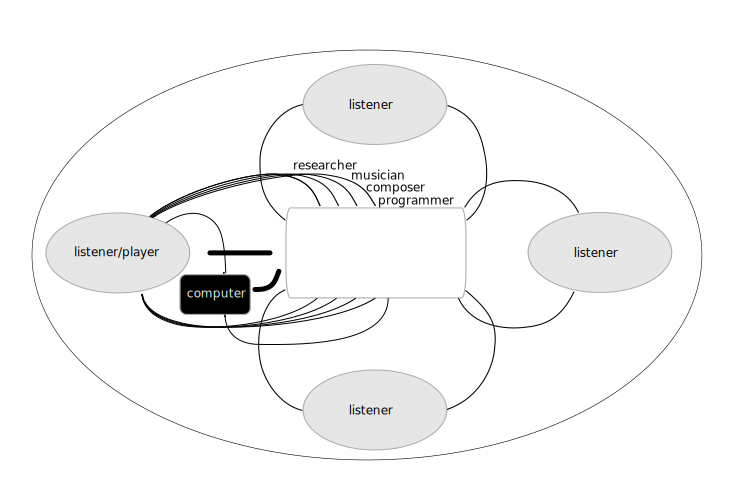
\includegraphics[width=\linewidth]{img/player-listener-computer}
  \caption{\small{A modified version of the previous graph (see Figure \ref{fig:player-comp}) where the listeners and the performer are united in the act of listening. A linear conception of a producer and a group of consumers is reduced in favor of a distributed sphere of listening.}}
  \label{fig:player-comp-2}
\end{figure}

In the graph representing a slice of time of a performance (see Figure \ref{fig:player-comp}), the trajectories of reflection create a feedback loop between the object of research and the musician. A corresponding loop may be found in between the listeners and the music representing the listener's reflections upon that same music as it takes place in real time. Although not likely to be entirely synchronous with those of the performer, provided the performer and the listeners share some musical references or have a common cultural ground, it is conceivable that some of the reflections made by the listeners overlap with some of the performer's. If I choose to play a note out of tune it is only if the significance of the `out-of-tuneness' is obvious to the listeners that they will appreciate it as something that adds to the music. If the significance of the pitch alteration is beyond reach it is more likely they will hear it as an error that maybe even reduces the value of the performance. It is as a listener I (as a performer) am able to reflect on that which I play---In a wider sense I am first a listener and then a performer since everything I play is a result of what I hear or have heard. Hence, the audible trace produced by me is an object for reflection common to both myself and the listener. In this view of our interactions the producer-consumer conception of performer-listener is resolved in favor of a relation more geared towards an  inter-subjectivity. Marcel \citeauthor{cobussen08}, in his book \citetitle{cobussen08}, discusses listening and suggests an understanding of ``listening to music'' that really means ``listening \emph{to and fro} music''.\footcite[p. 135 (italics by the author)]{cobussen08} When experienced, this oscillating movement of coming and going moves beyond the the idea of the listening subject and the sounding object. According to \citeauthor{cobussen08}, ``to listen to and fro decenters them, wipes them out.''\footcite[135]{cobussen08} Through the shared act of listening the subject-object divide between the listener and the sounding object is erased, and the producer-consumer distinction between the performer and the listener is blurred. 
If the performer is a listener among other listeners, the traditional view on a flow of communication from a (non-listening?) creator to a listening subject indeed becomes difficult to maintain. Instead we are presented with the image of a group of listeners in which some members are \emph{also} performers and creators (see Figure \ref{fig:player-comp}). I am not a performer that listens, I am a listener among other listeners that also performs. 

According to Vijay \citeauthor{iyer08} the sense of ``shared time'' is a property of music listening and is a crucial aspect of the temporality of performance. Listening to a performance of improvised music is to experience the improvisers real-time struggles, their in-time processes. Also to non-dance oriented music, listening to music is a co-performance, a ``participatory act of marking musical time with rhythmic bodily activity [which] physicalizes the sense of shared time, and could be viewed as embodied listening.''\footcite[276]{iyer08} Both in Cobussen's and Iyer's accounts, the interactions between the agents at play (listeners, performers, creators, etc.) are central. Not only what happens at each end of the flights of communication, but what happens \emph{between} the poles. Applied to the context of arts-based research this would mean to complement introspective reflections and reflections on the object with an investigation of what goes on in between these two poles (and between any other zones that influences the artistic practice). To attempt at unpacking the significance and impact of the low level interactions between oneself and ones surroundings.\footnote{Cf Chapter 11, in which the described project Bodies in Flight describes the contemporary human as \emph{an interstices in-between} various discursive fields and their related
technologies.} Furthermore, in the case of the time based arts, the temporalities of these interactions should be taken into account. The order of events as well as the temporal potential and prerequisites within the system(s) of interaction. (The temporality of the computer in Figure \ref{fig:player-comp} and \ref{fig:player-comp-2} is in every respect different from that of the listeners in the same figures.) But before turning to the aspect of multi-temporality within these interactions, I will again briefly turn to the nature of the in-time reflections in the imagined performance sketched in Figure \ref{fig:player-comp}.

In the interactions and feedback loops between the performer and the audible trace in Figures \ref{fig:player-comp} and \ref{fig:player-comp-2}, it is difficult to separate artistic evaluations and reflections from those that are research oriented. Or, perhaps more accurately described, also a research oriented reflection may very well result in an alteration of the object, an alteration that changes the music. The in-time research oriented reflection resists the theory versus practice divide in that it operates in parallel to the practice, and in that it undoubtedly also has an impact on that upon which it reflects.\footnote{Also compare to how Susanne Kozel earlier in this volume writes that ``innate to performance is the ability to reflect on what we are doing while we are doing it. I practice, and I reflect upon practice in infinitesimal loops.'' (Chapter 8, section 3, \S3} Not all art practice is arts-based research but all arts-based research performed in-time in the ways described here will alter the artistic expression in some respect. Also, the research activity may constitute meta-reflection, reflections upon purely musical reflections (e.g. \emph{Why is it important that this note is in tune?}) forming compound reflections of both artistic and research oriented nature further influencing the present and future expressive qualities of the creative work. In other words, although the trajectories of reflection may be distinct from one another, their responses are not. 

This perceptual non-linearity between cause and effect can also be found in the sometimes asymmetrical communications between a performer, an interactive computer system, and listeners. Imagine a performance where the computer `listens' to the performer and responds to a given set of triggers (a particular note, a gesture, a rhythm, etc.). Imagine further that in the performance the system fails at recognizing a particular trigger, with the effect that the desired response is not achieved. This `mistake' is likely to alter the music. Not only because the desired response was not triggered, but also because the performer, in response to the missed cue, may alter the playing in order to facilitate the computer recognition (play the triggering phrase louder, slower, shorter or faster, etc). A reflection upon past and current events in one domain (\emph{``the computer missed my cue''}), induces a change in another, which in turn may lead to altered decisions in yet a third domain (\emph{``I should re-write the program''}). Although the same scenario could happen between two human performers, even if we disregard the comparatively limited interactive potential with the computer, its temporality makes the human-computer interaction distinct from human-human interaction. 
%The trajectories of reflection upon the missed cue, and its consequences, cause changes in the system which may not easily be traced back to the cause. 
%The differing modalities of reflection, which have their roots in differing temporalitites, may create a breach between the perception of the event and its cause. 

The different temporalities of the elements involved in an interactive performance such as the one described here are important to understand and acknowledge for the art based researcher. A computer, as a concept and before engaged in an interactive performance, may be seen as the ultimate representation of time as space. Its operations are almost entirely independent of time. Hence writing computer programs to be used in interactive performances is a difficult task, and using them is even more daunting. The need to understand and evaluate the changes, and the reason for the changes, in the computer output, is without a doubt one of the more challenging aspects of being a computer musician. It involves having to evaluate abstract and largely outside-of-time functionality of a computer program in performance while simultaneously engaging in the temporal flux of the in-time progress of the music. But in the process some aspects of the complexity of the multi-temporal capacity in the performer-listener feedback loops sketched above is revealed

A computer program written to perform in an interactive performance may have pre-conceived structures not unlike a musical composition or a structured improvisation and writing such a program is an over-time process similar to how composing is an over-time process. Furthermore writing a musical composition and performing it involves similar kinds of tensions between over-time and in-time decisions that may be found in the performance with an interactive computer. Now, whereas a musical score is not easily changed during a performance,\footnote{To be fair, any performed composition is altered by its performance in one way or another, but, in the Western art music tradition, radical in performance alterations of the written music are more likely to be called mistakes rather than interpretation.} in the case of the interactive computer, whatever the agenda used to construct the program, if the interaction is successfully exploited, the agenda may be altered. Not only in the performance but \emph{by} the performance. But this can of course only be true if we resist and challenge the simplicity of the click-and-response interaction discussed above (see Section \ref{sec:why-interaction}) and take full account of time and memory.

% The asymmetry in the trajectories of reflection discussed above is % also mirrored in the performer-computer-listener interactions. The % musical in-time evaluation on a series of events emanating from the % computer, made without knowledge of, or interest in their origin (i.e. % the musician's particular interaction with the computer), will not % necessarily correspond to an evaluation of the same events from % \emph{within} the process. The consequence may be that, in a response % to the performer's reflection, a change is introduced in the output % that, to a listener, who is primarily concerned with the audible % trace, and may be unaware or unconcerned with the details of the % musician-computer interaction, sounds awkward. The differing % modalities of reflection which have their roots in differing % temporalitites, creates a breach between the listener and the % performer. The temporal differences is one aspect of the issue at % stake here, but it is not the only one. 
% Due to a poor performance, bad programming or some other factor the % virtuality of the computer instrument fails to reveal itself and the % musical decisions made by the performer becomes enigmatic to the % listener.
% Either way,
The use of the computer in live performance shows that in-time and over-time processes are not mutually exclusive. They can co-exist but their zones of interaction may also result in noise and a distorted perception. The ``shared time'' of music listening is created through the performer-computer-listener feedback loops. To hold different temporal representations active at the same time may be second nature for a musician, but the added aspect of the interactive computer makes it both more complex to understand and more difficult to perform, but it may also help the performer-researcher to understand and acknowledge the different temporal modes in operation.





\section{Interacting with the Virtual}
\label{sec:inter-with-virt}

The almost mystical sensation of simultaneously being able to be in time, `now' and in memory, in the recollection of a previous now, is an important and powerful aspect of time-based arts in general and music in particular. Imagine listening to a well known melody being played. As the melody is unfolding there is a perpetual interaction between its in-memory representation and its real-time representation. Sometimes, if the memory of a particular music is really strong, it may overshadow the real life version of it and inversely, if the performance is powerful and expressive it may smear out the original memory, overwriting it with the new version. As was discussed above, it is tempting, and practical, to gather musical events into larger structures (e.g. notes into melodies, movements into symphonies, songs into song-cycles, etc.) and regard them as singularities, as image representations of what they represent. As such they would have no reference to time, their temporality gets transformed to a kind of spatiality. Conceptually they would approach the ideal mathematical formula and become a representation of \emph{infinite time},\footcite{roads} or, to put it in Xenakis' words, time is abolished in such structures: ``[O]ne could say that every temporal schema, pre-conceived or post-conceived, is a representation outside time of the temporal flux in which the phenomena, the entities, are  inscribed''.\footcite[264]{xenakis71} They become spatial, and virtual, translations of the original in-time representations. If time really is abolished, how is is that we can keep track of such time specific data as duration, and silence, in memory representations of music? The question is not merely of theoretical or philosophical import, it has great impact on the way we understand and execute Practice based Research in the real-time arts. To examine a musical practice from within---as opposed to examining it from the outside---we need to be able to access the object in real-time. And to gain access to it in real-time it is necessary to understand what real-time is relative to non real-time, i.e. in-memory representations.

In the survey of memory and imagination in Paul Ric{\oe}ur's seminal book \citetitle{ricoeur04} among many other things in the first chapter, he critically discusses Husserl's concept of memory in general and the ideas of \emph{retention} in particular.\footnote{The full meaning of this concept and the significance of Ric{\oe}ur's thinking upon it is far beyond the scope of this chapter. I use these sources as inspiration and I do not intend to unwrap a full philosophical discussion on time.} The duration of a musical note is used to address the question of what it means for something that endures to remain. And this is indeed at the heart of the matter for the present discussion: When in music, or any other real-time art form, we perform there is a complex interplay between creation and duration. Musicians do not only play series of instances that are sequentially combined, they play notes, phrases and gestures that have a duration. These entities can be accessed by the performer as a series of instants, or sub-entities, but also as a unity, a whole, that may signify something far beyond the sum of its parts. Something which has both a virtual, in memory, and a real representation. These entities endure and as they develop in time, they create duration.

How is this possible? How can the present `now' and the memory of the past `nows' coexist? How can the memory of the preceding now co-exist with the memory of a now six months ago? Husserl, with the sounding note as an example, states that a musical note as it is played makes the now perceptible, and, as it continues to sound it ``has an ever new now, and the now that immediately precedes it changes into a past.''\footcite[\emph{Vorlesungen zur Phänomenologi des inneren Zeitbewussteins}, Husserl, E. cited in][32]{ricoeur04} The `ever new now' is what constitutes the modification in the perception that constructs the duration. The `now' that is pushed back by the `new' now however is not disappearing but is held on to, and it is this `holding on to' that Husserl labels \emph{retention}.\footcite[32]{ricoeur04} Hence retention is, in a manner of speaking, a way to hold on to the note while it is sounding. It is not its memory, or recollection, but its modified perception. Neither is retention and imagination the same thing. And although the retention of a note and its present `now' are not the same thing, together they constitute the experience of the note as a whole, as a duration. But as long as the retention lasts ``the tone has its own temporality''. Retention is a modification of perception and the difference between them is first and foremost a temporal one. Perhaps it is possible to imagine an interaction between retention and  recollection. While holding past `nows' of that which is unfolding in time in retention one can simultaneously recollect previous instances of the same expression (a note, a phrase, a gesture, etc) and compare the two. While the `now' continuously begins and recedes, with past nows sinking into retention, recollections rise from below and create a virtual now parallel to the real now. A new now that can never become the `real' but one which can trail the present. It can be experienced almost as if it took place in the real domain. A virtual (re-)presentation moving alongside of, or being pulled by, the real in a continuous flow in time. The real and the virtual as sketched above may be seen as modes of listening: Outwards, listening to one's own or others' sounds as they disclose in time and inwards, listening to past experiences and memory representations. Both of these modes continuously co-exist and interact with each other.\footnote{These ideas are loosely related to how Susanne Kozel states that ``in every creative project there is an invisible'' (Chapter XX, Section \emph{Material Ontology} \S6). Henk Borgdorff's similarly speaks of a reality of the art work that ``precedes any re-presentation in the space of the conceptual.'' (Chapter XX, Section \emph{Some remarks on the epistemology...}, \S8)}

% In practice the musician can not lean on only one of these modes but % must let both the real and the virtual listening modes % co-exist.\footnote{See also Susan Kozel's chapter in this Volume % Section \emph{Material Ontology} \S6.}

According to Henri Bergson we can look at the present-past axis as an inverted cone (think an ice-cream cone) where the tip is the present and the base represents the oldest unconscious memories. Each segment of this cone, where a segment is a line trisecting it somewhere between its point and its base, represents a virtual plane, a region in the past.\footcite[][Ch.3]{bergson91} 
In Gilles Deleuze's reading of Bergson each such region contains the totality of the past in different levels of contraction or relaxation and at any time we can make a leap to any segment of the cone, to any past memory, bringing it back into consciousness.\footcite[][60]{deleuze88} The cone is not to be understood as a storage device in which memories are put, slice by slice in succession, but rather it is an abstract visualisation of the human capacity to place oneself in the past, while still having access to everything prior to that particular point in time, as well as everything past it: ``It is in this sense that one can speak of the regions of Being itself, the ontological regions of the past `in general', all coexisting, all repeating one another.''\footcite[61]{deleuze88}
The cone symbolizes a dynamic process, more dynamic than what the image can represent, for there are several motions in simultaneous operation. The tip of the cone, which at all times represents the present moves perpetually along the plane of existence, ``of my actual representation of the universe'' all while the base of the cone remains still. If this is the horizontal movement there are corresponding vertical movements where pure memories are descending down to the tip, to where action takes place, and images from the present are ascending up into memory.\footcite[See also][47-8]{lawlor03} In other words, we have two contrasting movements, one of the cone moving on the plane and one inside the cone affecting the level of contraction at any virtual plane within the cone. Hence the virtual plane of memory is not a static \emph{image} (space) of a time in the past (a sound), but a constantly changing one. Following this conceptualization of the relation between the present and the past, the idea of a temporal schema outside of time that Xenakis brought forth should perhaps be questioned. In my own experience as a performer, the memory of a musical event vividly holds on to the temporal aspect of its origin. My memory of it is a memory, not outside of time, because the temporal relations between the events contained in it matters to the actual memory.

\begin{figure}[htb]
  \centering
  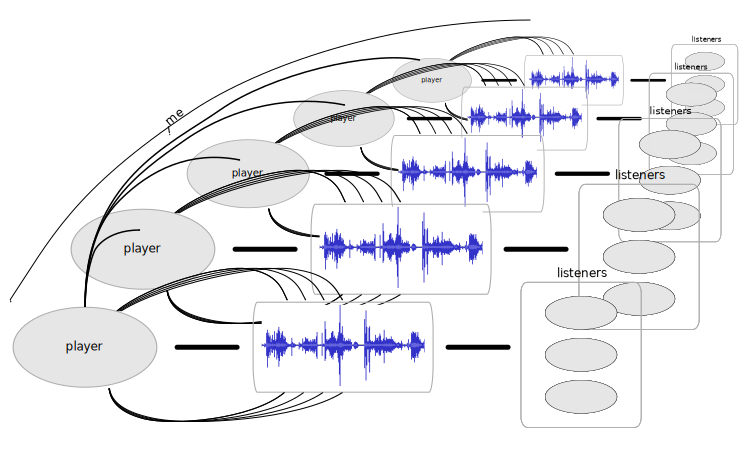
\includegraphics[width=\linewidth]{img/players-perspective}
  \caption{The imaginary performance as sketched in Figure \ref{fig:player-comp} with the addition of time. Past events are fading out but held on to by the in-time performer as is represented by the arrows pointing back unto previous nows. It should be noted that this is a extremely simplified graphic representation of phenomena that are infinitely more complex.}
  \label{fig:u}
\end{figure}

These virtual planes of memory are likely to be linked to the virtuality present in all musical creation. Common to both the virtual planes of memory and to the virtuality of music is that, although they generate visual elements and images, they do not depend on them.
But in real-time performance, in improvisation---in the spur of the moment---the leap from `now' to a virtual plane of the past may create a breach similar to how musical decisions made based on information hidden from the listener creates a breach, as was discussed above. An ontological difference that, in the best case, fuels a musical performance and takes it to new heights, but at its worst, detaches the performance from the logic of the `now', and the virtual plane fails to actualize itself and remains trapped in the memory of the performer(s). These leaps may be carried out as a result of affectivity within the performer or simply by aesthetic choices.

In Figure \ref{fig:u} the slice of time discussed earlier is now put into the context of the flow of time. Past events are slowly sinking into retention but the reflective listener-performer is able to make a leap back in time. Although only the activities of the performer are plotted, similar leaps back in time are obviously also performed by any given listener.

\section{Summary}
\label{sec:summary}

The distinction between in-time and over-time processes in art is obviously not clear cut. Most art practice, as has already been pointed out, begin with some kind of over-time process in its stage of preparation. Even improvisatory practices, which depend extensively on in-time activities, commonly involve stages of preparation in which constraints and  limitations are set up. By introducing the interactive computer in this context the over-time articulations (artistic structures, constraints, form, etc.) may be brought into real-time performance, hence a layer of complexity is added for both the performer and the researcher. In the words of Susanne Kozel\footnote{See Chapter XX: The Virtual and the Physical, Section ``The constrainst and urgencies of practice'', \S1} the computer may provide a structure that, in the interactions with a performer, constructs ``a topology of meaning'': In itself a valid metaphor for the holistic nature of the interactions between in-time and over-time processes that has been discussed throughout this chapter.

Music has had an out-of-time spatial representation ever since musical notation was introduced. In the Western music history there is a tendency of disregarding the performative aspects of a musical work and regarding the score, i.e. its graphical representation, as equal to the identity of the work.\footnote{The topic is brought up by British improviser and composer Trevor Wishart who rhetorically asks what constitutes music: ``what we experience in the sounds, or what we might theoretically appreciate of the score through the sounds [\ldots].'' \cite{wis96}} Furthermore, with the advent of recording technology, not only the representation of sound in scores, but also sound itself was transformed into space: ``We might say that recording is a reflux, or distillation in which time is boiled off, for time must be added back in to get sound, in the form of a steady motion of the turntable or tape heads or the crystal clock in digital recording.''\footcite[54][]{evens05} In the engravings on an LP, or through the holes on the surface of a CD, the elusive nature of sound as embedded in time is captured and spatialized. The digital representation of sound in a computer is similarly spatialized: In other words, to even begin to think about using interactive computer technology in performance involves a transformation of the in-time embedded sound to an over-time representation.

In his book \citetitle{dixon07} Steve Dixon discusses the problematic issue of `liveness' in performance. There is a common sense that technology have ``transformed or destabilized notions of liveness, presence, and the `real''',\footcite[127]{dixon07} suggesting that the real-time arts somehow becomes less `live' when technology is made use of. Similar ideas have been discussed in this chapter based on the notion that it is the temporality of technology that is different from the temporalities of live performance. Even though a performer (and an audience), simultaneously employs a number of different temporalities (as was discussed in Section \ref{sec:performing-time}), the addition of the computer appears to disrupt the in-time process in various ways. As if the non-temporality of the computer was too much for the performance to carry, making it impossible for the interactive interface to inform the digital system in a useful way. Although the problem as it is described here is particular to the field or artistic practice, any knowledge produced about why the interface fails, and how it may be improved in this context, will be of interest, and of potential use, also outside of that field. The significance of arts-based research in this context has at least two axes: (1) to more fully understand the notion of liveness and temporal embeddedness and (2) to inform the design of a less disruptive performer-computer interface.

Over the last three or four decades a number of successful interactive art works have been produced, surpassing the limitations and quirks of digital systems. The ideal interactive performance system will (should) hide its abstract functionality, its dependence on \emph{states} rather than dynamic changes in a constant flux, from the user/performer, and by doing so it will also conceal its structure. Furthermore, a successful interaction with the computer may create the impression that the computer is indeed acting dynamically, intelligently adopting its state according to past and present input. While this may be said to be true today, present day human-computer interaction can only be compared to human-human interaction if the notion of the latter is infinitely reduced. Nothing is gained by pretending that interactive computers in the context of real time performance are even comparable to the interactive potential in a human performer. On the opposite will we risk at reducing the meaning of concepts like `interaction', and `intelligent systems' into pointless concepts with nothing but potential market value. However, arts-based research in the context of the real-time arts, because of its high demands and its largely non-traditional methods, has great potential to inform the  more general field of Human Computer Interaction research. There is a tendency to limit the thinking about HCI to ``microlevel interactions between programmers or users and computers. The broader social forces and structures that constrain such interactions and are themselves reproduced and molded by microlevel events are often left unexamined.'' arts-based research in the real-time arts has much to contribute here and may provide a useful alternative to the  ``naive image of human-computer interaction as narrowly technical and as a problem of cognitive optimization''.\footcite[325]{engestrom96} In particular in the ways that time and memory is represented and in the ways that the abstract, non-temporality of the computer has to be tackled. 

%That the practice of artists in the real-time arts may be of interest to a wide range of research disciplines 

% The virtuality of digital technologies is comparable, both in scope % and in force, to the virtuality of the art work. 


%%%%%%%%%%%%%%%%%%%%%%%%%%%%%%%%%%%%%%%%%%%%%%%%%%
%%%%%%%%%%%%%%%%%%%%%%%%%%%%%%%%%%%%%%%%%%%%%%%%%%

It will always be tempting to approach the object of research as a whole rather than as a distributed agglomeration of interconnected slices in time. Throughout this chapter I have argued that the interaction between in-time and over-time aspects of the artistic practice is of great significance. Furthermore, I have stressed that the use of interactive computer technology is of interest to the topic of arts-based research in that it surfaces issues pertaining to time and temporalities in the context of real time arts, but also in the ways it offers connections to adjoining research disciplines. The memory image of an in-time process as a time spectrum; a spatial transformation in which time is abolished is questioned.

turning to Bergson's theories on time and memory.

% While the ontology of the Western musical work to some extent rests on % an understanding of the work outside of time, I argue that arts-based research should % approach 

% describing what it is rather than how it came into being. Describing % its idealized meaning rather than the sometimes banal interactions % that participated in its construction. 

% Non-temporal representations are easier to document and easier to % comment upon. 
% Though Xenakis claims that a transformation from time to space is % possible, suggesting the possibility of an in memory image % representation of an in-time process. 

% However, by introducing Bergson's theories on time and memory and % linking these to the in-time processes of I have attempted to show % that not even the in-memory, seemingly non-temporal representation of % musical flow appears to exist outside of time. In this connections % lies an openingfor arts-based research in the temporal arts to investigate its objects % without falling back on musical notation or fully non-temporal modes % of representation. These investigation, I believe, will be potentially % very interesting to other artistic disciplines such as film and % theater, but also to non-arts based sciences like cognitive sciences % and physics.

%Traditional musicological research commonly resorts to non-temporal representations of the music it attempts to investigate such as musical notation.


\section{Coda}
\label{sec:coda}

In a commentary to the opening quote from Wagner's Parsifal, German composer Wolfgang Rihm points out the brilliance in the way Wagner stages the time to space transformation. It is not made by a sudden move but rather as a seemless transition, like a walk through a long series of infinitesimal transformations. (Along with the music Gurnemanz and Parsifal are slowly walking backs turned to the audience.) When portraying the time to space transition, Wagner resists the non-temporal aspect of space, and focuses on the movement, for, as Rihm states, the perception of space requires movement.\footcite{rihm01} To Rihm time is movement. In a constant motion, events are sinking into time (similar to how the concept of retention was described above), and in the process that which we label musical material is constructed. If musicological research has been focused on describing that material, arts-based research should, among other things, concern itself with the motion that precedes it.



% ``Composition liberates time so that it can be lived, not % stockpiled.''\footcite[][145]{attali85}

% But with the spatialisation of sound came also the possibility for an % unprecedented temporal precision.\footcite[4]{moore90} A precision % which allowed for the study of sound, for microsound,\footcite{roads} % and for scientific repeatability. To relocate the stockpiled, % spatialized sound from its over-time representations to its in-time % representation and perform the study of it in that domain, is one of % the great challenges of arts-based research. 

% And in this transformation, music was commodified.

% In the way I (freely) interpret Attali's short statement it is an urge % to engage in the 

%  Within the field of Human Computer Interaction research there has % been a tendency to limit the thinking about 

%  That in a succesful interaction with a computer the user/performer % will merge with the system and make it dynamic. 


% That this fact should be the driving force behind all interactive % systems designs.

% Furthermore, by introducing the interactive computer in performance % the matter is both complicated and simplified. From 

% the aspects of multiple simultaneous temporalities in the way 
% the researcher can gain access to 


% Using interactive computers in performance is a way to bring the % complexities of the in-time and over-time interactions to the % forefront.

%%% Local Variables: 
%%% mode: latex
%%% TeX-master: "InteractivityTimeSpace"
%%% End: 
